% Options for packages loaded elsewhere
\PassOptionsToPackage{unicode}{hyperref}
\PassOptionsToPackage{hyphens}{url}
%
\documentclass[
  ignorenonframetext,
]{beamer}
\usepackage{pgfpages}
\setbeamertemplate{caption}[numbered]
\setbeamertemplate{caption label separator}{: }
\setbeamercolor{caption name}{fg=normal text.fg}
\beamertemplatenavigationsymbolsempty
% Prevent slide breaks in the middle of a paragraph
\widowpenalties 1 10000
\raggedbottom
\setbeamertemplate{part page}{
  \centering
  \begin{beamercolorbox}[sep=16pt,center]{part title}
    \usebeamerfont{part title}\insertpart\par
  \end{beamercolorbox}
}
\setbeamertemplate{section page}{
  \centering
  \begin{beamercolorbox}[sep=12pt,center]{part title}
    \usebeamerfont{section title}\insertsection\par
  \end{beamercolorbox}
}
\setbeamertemplate{subsection page}{
  \centering
  \begin{beamercolorbox}[sep=8pt,center]{part title}
    \usebeamerfont{subsection title}\insertsubsection\par
  \end{beamercolorbox}
}
\AtBeginPart{
  \frame{\partpage}
}
\AtBeginSection{
  \ifbibliography
  \else
    \frame{\sectionpage}
  \fi
}
\AtBeginSubsection{
  \frame{\subsectionpage}
}
\usepackage{amsmath,amssymb}
\usepackage{iftex}
\ifPDFTeX
  \usepackage[T1]{fontenc}
  \usepackage[utf8]{inputenc}
  \usepackage{textcomp} % provide euro and other symbols
\else % if luatex or xetex
  \usepackage{unicode-math} % this also loads fontspec
  \defaultfontfeatures{Scale=MatchLowercase}
  \defaultfontfeatures[\rmfamily]{Ligatures=TeX,Scale=1}
\fi
\usepackage{lmodern}
\usetheme[]{Madrid}
\usecolortheme{dolphin}
\ifPDFTeX\else
  % xetex/luatex font selection
\fi
% Use upquote if available, for straight quotes in verbatim environments
\IfFileExists{upquote.sty}{\usepackage{upquote}}{}
\IfFileExists{microtype.sty}{% use microtype if available
  \usepackage[]{microtype}
  \UseMicrotypeSet[protrusion]{basicmath} % disable protrusion for tt fonts
}{}
\makeatletter
\@ifundefined{KOMAClassName}{% if non-KOMA class
  \IfFileExists{parskip.sty}{%
    \usepackage{parskip}
  }{% else
    \setlength{\parindent}{0pt}
    \setlength{\parskip}{6pt plus 2pt minus 1pt}}
}{% if KOMA class
  \KOMAoptions{parskip=half}}
\makeatother
\usepackage{xcolor}
\newif\ifbibliography
\usepackage{color}
\usepackage{fancyvrb}
\newcommand{\VerbBar}{|}
\newcommand{\VERB}{\Verb[commandchars=\\\{\}]}
\DefineVerbatimEnvironment{Highlighting}{Verbatim}{commandchars=\\\{\}}
% Add ',fontsize=\small' for more characters per line
\usepackage{framed}
\definecolor{shadecolor}{RGB}{248,248,248}
\newenvironment{Shaded}{\begin{snugshade}}{\end{snugshade}}
\newcommand{\AlertTok}[1]{\textcolor[rgb]{0.94,0.16,0.16}{#1}}
\newcommand{\AnnotationTok}[1]{\textcolor[rgb]{0.56,0.35,0.01}{\textbf{\textit{#1}}}}
\newcommand{\AttributeTok}[1]{\textcolor[rgb]{0.13,0.29,0.53}{#1}}
\newcommand{\BaseNTok}[1]{\textcolor[rgb]{0.00,0.00,0.81}{#1}}
\newcommand{\BuiltInTok}[1]{#1}
\newcommand{\CharTok}[1]{\textcolor[rgb]{0.31,0.60,0.02}{#1}}
\newcommand{\CommentTok}[1]{\textcolor[rgb]{0.56,0.35,0.01}{\textit{#1}}}
\newcommand{\CommentVarTok}[1]{\textcolor[rgb]{0.56,0.35,0.01}{\textbf{\textit{#1}}}}
\newcommand{\ConstantTok}[1]{\textcolor[rgb]{0.56,0.35,0.01}{#1}}
\newcommand{\ControlFlowTok}[1]{\textcolor[rgb]{0.13,0.29,0.53}{\textbf{#1}}}
\newcommand{\DataTypeTok}[1]{\textcolor[rgb]{0.13,0.29,0.53}{#1}}
\newcommand{\DecValTok}[1]{\textcolor[rgb]{0.00,0.00,0.81}{#1}}
\newcommand{\DocumentationTok}[1]{\textcolor[rgb]{0.56,0.35,0.01}{\textbf{\textit{#1}}}}
\newcommand{\ErrorTok}[1]{\textcolor[rgb]{0.64,0.00,0.00}{\textbf{#1}}}
\newcommand{\ExtensionTok}[1]{#1}
\newcommand{\FloatTok}[1]{\textcolor[rgb]{0.00,0.00,0.81}{#1}}
\newcommand{\FunctionTok}[1]{\textcolor[rgb]{0.13,0.29,0.53}{\textbf{#1}}}
\newcommand{\ImportTok}[1]{#1}
\newcommand{\InformationTok}[1]{\textcolor[rgb]{0.56,0.35,0.01}{\textbf{\textit{#1}}}}
\newcommand{\KeywordTok}[1]{\textcolor[rgb]{0.13,0.29,0.53}{\textbf{#1}}}
\newcommand{\NormalTok}[1]{#1}
\newcommand{\OperatorTok}[1]{\textcolor[rgb]{0.81,0.36,0.00}{\textbf{#1}}}
\newcommand{\OtherTok}[1]{\textcolor[rgb]{0.56,0.35,0.01}{#1}}
\newcommand{\PreprocessorTok}[1]{\textcolor[rgb]{0.56,0.35,0.01}{\textit{#1}}}
\newcommand{\RegionMarkerTok}[1]{#1}
\newcommand{\SpecialCharTok}[1]{\textcolor[rgb]{0.81,0.36,0.00}{\textbf{#1}}}
\newcommand{\SpecialStringTok}[1]{\textcolor[rgb]{0.31,0.60,0.02}{#1}}
\newcommand{\StringTok}[1]{\textcolor[rgb]{0.31,0.60,0.02}{#1}}
\newcommand{\VariableTok}[1]{\textcolor[rgb]{0.00,0.00,0.00}{#1}}
\newcommand{\VerbatimStringTok}[1]{\textcolor[rgb]{0.31,0.60,0.02}{#1}}
\newcommand{\WarningTok}[1]{\textcolor[rgb]{0.56,0.35,0.01}{\textbf{\textit{#1}}}}
\usepackage{graphicx}
\makeatletter
\def\maxwidth{\ifdim\Gin@nat@width>\linewidth\linewidth\else\Gin@nat@width\fi}
\def\maxheight{\ifdim\Gin@nat@height>\textheight\textheight\else\Gin@nat@height\fi}
\makeatother
% Scale images if necessary, so that they will not overflow the page
% margins by default, and it is still possible to overwrite the defaults
% using explicit options in \includegraphics[width, height, ...]{}
\setkeys{Gin}{width=\maxwidth,height=\maxheight,keepaspectratio}
% Set default figure placement to htbp
\makeatletter
\def\fps@figure{htbp}
\makeatother
\setlength{\emergencystretch}{3em} % prevent overfull lines
\providecommand{\tightlist}{%
  \setlength{\itemsep}{0pt}\setlength{\parskip}{0pt}}
\setcounter{secnumdepth}{-\maxdimen} % remove section numbering
\ifLuaTeX
  \usepackage{selnolig}  % disable illegal ligatures
\fi
\IfFileExists{bookmark.sty}{\usepackage{bookmark}}{\usepackage{hyperref}}
\IfFileExists{xurl.sty}{\usepackage{xurl}}{} % add URL line breaks if available
\urlstyle{same}
\hypersetup{
  pdftitle={Causal Inference and Machine Learning},
  hidelinks,
  pdfcreator={LaTeX via pandoc}}

\title{Causal Inference and Machine Learning}
\subtitle{In Economics, Social, and Health Sciences
\newline \smallskip \textit{by Mutlu Yuksel and Yigit Aydede}}
\author{}
\date{\vspace{-2.5em}}

\begin{document}
\frame{\titlepage}

\begin{frame}{From Data to Causality: Alex's Allergy Story}
\protect\hypertarget{from-data-to-causality-alexs-allergy-story}{}
\begin{itemize}
\tightlist
\item
  Alex collects data on meals and symptoms
\item
  Uses \textbf{visualizations} to explore relationships
\item
  Forms hypotheses about garlic as the cause
\end{itemize}

\note{
Use this relatable example to introduce students to observational data, correlation, and the transition to causality.
}
\end{frame}

\begin{frame}{Visual Tools Alex Used}
\protect\hypertarget{visual-tools-alex-used}{}
\begin{itemize}
\tightlist
\item
  \textbf{Histogram} of reaction intensity
\item
  \textbf{Bar Chart}: reactions by food type
\item
  \textbf{Time Series}: reactions over time
\end{itemize}

\emph{(Insert example figures here from saved outputs)}

\note{
Encourage students to describe what each plot shows and how it supports hypothesis generation.
}
\end{frame}

\begin{frame}[fragile]{Quantifying Correlation}
\protect\hypertarget{quantifying-correlation}{}
\begin{itemize}
\tightlist
\item
  Alex notices garlic has high correlation with intense reactions
\item
  Some spurious patterns: weekends linked with reactions due to dining
  out
\end{itemize}

\begin{Shaded}
\begin{Highlighting}[]
\FunctionTok{cor}\NormalTok{(data}\SpecialCharTok{$}\NormalTok{garlic, data}\SpecialCharTok{$}\NormalTok{reaction\_intensity)}
\end{Highlighting}
\end{Shaded}

\note{
Introduce idea of correlation coefficients and explain what “spurious correlation” means in practical terms.
}
\end{frame}

\begin{frame}[fragile]{Controlling for Confounders with Regression}
\protect\hypertarget{controlling-for-confounders-with-regression}{}
Alex estimates:

\begin{Shaded}
\begin{Highlighting}[]
\NormalTok{model }\OtherTok{\textless{}{-}} \FunctionTok{lm}\NormalTok{(reaction\_intensity }\SpecialCharTok{\textasciitilde{}}\NormalTok{ garlic }\SpecialCharTok{+}\NormalTok{ weight }\SpecialCharTok{+}\NormalTok{ temperature }\SpecialCharTok{+}\NormalTok{ outside, }\AttributeTok{data =}\NormalTok{ data)}
\FunctionTok{summary}\NormalTok{(model)}
\end{Highlighting}
\end{Shaded}

\begin{itemize}
\tightlist
\item
  Holds constant other variables
\item
  Finds garlic still strongly predicts symptoms
\end{itemize}

\note{
Explain that OLS helps isolate garlic’s effect while controlling for weight, temperature, etc.
}
\end{frame}

\begin{frame}{Experimental Design to Identify Causality}
\protect\hypertarget{experimental-design-to-identify-causality}{}
\begin{itemize}
\tightlist
\item
  Alex and friends eat same meals (some with garlic)
\item
  Only Alex shows symptoms
\item
  Confirms garlic as causal trigger
\end{itemize}

\note{
Use this slide to introduce randomization, control groups, and the strength of experimental evidence.
}
\end{frame}

\begin{frame}{Spurious Correlation: Mia's Story}
\protect\hypertarget{spurious-correlation-mias-story}{}
\begin{itemize}
\tightlist
\item
  Mia gets sick on garlic days too
\item
  Turns out: it's the \textbf{candle} causing her reactions
\item
  Not garlic → \textbf{confounding by context}
\end{itemize}

\note{
Great moment to discuss omitted variable bias and the risk of misattributing causes in observational data.
}
\end{frame}

\begin{frame}{From Correlation to Causation}
\protect\hypertarget{from-correlation-to-causation}{}
\begin{itemize}
\tightlist
\item
  Step 1: Observe patterns in data
\item
  Step 2: Control for confounders
\item
  Step 3: Test causality experimentally
\item
  Step 4: Rule out alternative explanations
\end{itemize}

\note{
Wrap up Alex & Mia's journey as a metaphor for applied causal inference.
}
\end{frame}

\begin{frame}{Qualitative vs.~Quantitative Research}
\protect\hypertarget{qualitative-vs.-quantitative-research}{}
\begin{itemize}
\tightlist
\item
  \textbf{Qualitative}: interviews, focus groups, documents
\item
  \textbf{Quantitative}: surveys, statistical models, structured data
\end{itemize}

\note{
Discuss inductive vs. deductive logic. Emphasize that both methods are valuable but serve different purposes.
}
\end{frame}

\begin{frame}{Data and Visualization}
\protect\hypertarget{data-and-visualization}{}
\begin{itemize}
\tightlist
\item
  Visualization helps generate hypotheses
\item
  Patterns can be misleading if not contextualized
\end{itemize}

\note{
Remind students that before modeling, it's critical to “look at your data.”
}
\end{frame}

\begin{frame}{Anscombe's Quartet: Why Visualization Matters}
\protect\hypertarget{anscombes-quartet-why-visualization-matters}{}
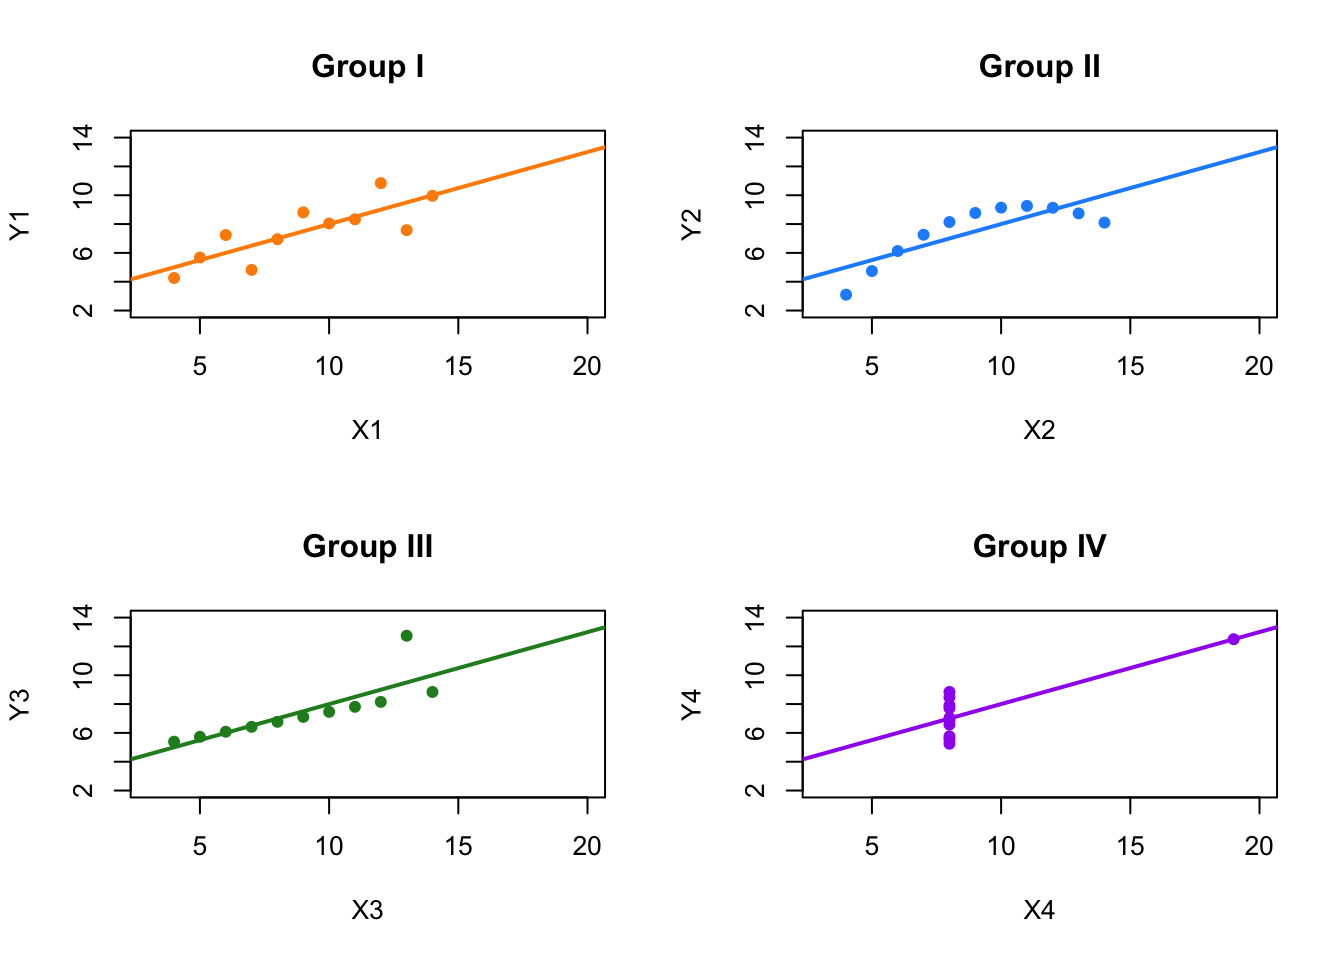
\includegraphics[width=0.8\textwidth,height=\textheight]{anscombe-plot-1.png}

\begin{itemize}
\tightlist
\item
  Same mean, variance, correlation, and regression line\\
\item
  Different visual patterns → Different data stories
\end{itemize}

\note{
A powerful example showing why summary stats alone aren’t enough.
}
\end{frame}

\begin{frame}{Nonlinear Relationships}
\protect\hypertarget{nonlinear-relationships}{}
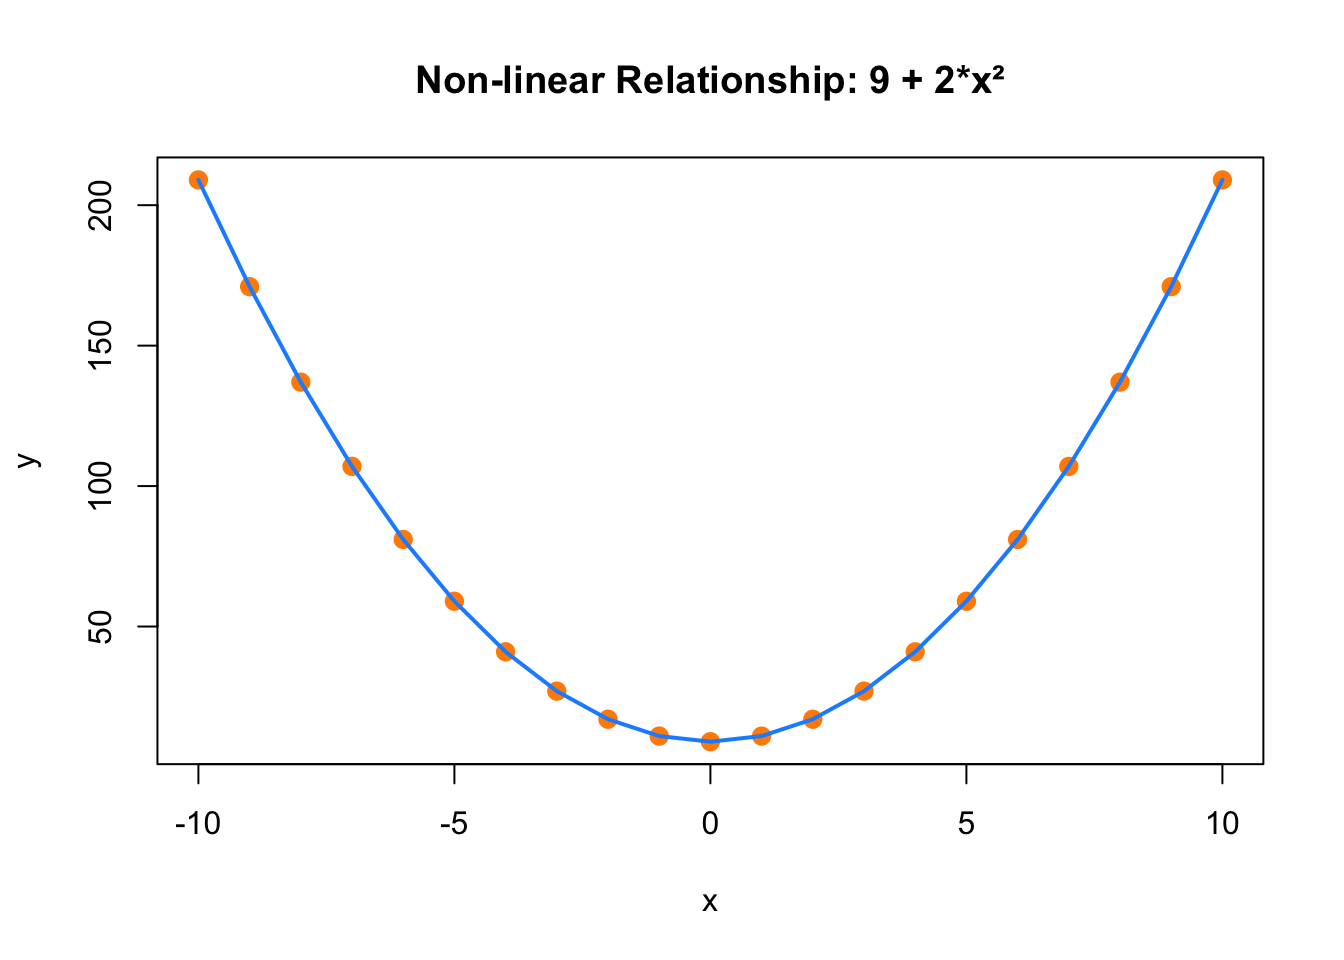
\includegraphics[width=0.7\textwidth,height=\textheight]{nonlinear-plot-1.png}

\begin{itemize}
\tightlist
\item
  Correlation may be high, but linear regression fails
\item
  Nonlinearity is a common reason for poor model fit
\end{itemize}

\note{
Discuss functional form misspecification. Ask what would happen if we fit a straight line here.
}
\end{frame}

\begin{frame}{Correlation and Regression}
\protect\hypertarget{correlation-and-regression}{}
\begin{itemize}
\tightlist
\item
  Correlation measures association, not direction of effect
\item
  Regression allows prediction and controlling for other variables
\end{itemize}

\note{
Use this to transition toward regression and causal thinking.
}
\end{frame}

\begin{frame}{The Effect of \(X\) on \(Y\)}
\protect\hypertarget{the-effect-of-x-on-y}{}
We want to model:

\[
Y = \beta_0 + \beta_1 X + \varepsilon
\]

\begin{itemize}
\tightlist
\item
  \(Y\): outcome\\
\item
  \(X\): predictor\\
\item
  \(\varepsilon\): unobserved error
\end{itemize}

\note{
Introduce the linear model. Emphasize goal: estimate \(\beta_1\) accurately.
}
\end{frame}

\begin{frame}[fragile]{Estimating \(\beta_0\) and \(\beta_1\)}
\protect\hypertarget{estimating-beta_0-and-beta_1}{}
\begin{Shaded}
\begin{Highlighting}[]
\NormalTok{b1 }\OtherTok{\textless{}{-}} \FunctionTok{cov}\NormalTok{(x, y) }\SpecialCharTok{/} \FunctionTok{var}\NormalTok{(x)}
\NormalTok{b0 }\OtherTok{\textless{}{-}} \FunctionTok{mean}\NormalTok{(y) }\SpecialCharTok{{-}}\NormalTok{ b1 }\SpecialCharTok{*} \FunctionTok{mean}\NormalTok{(x)}
\end{Highlighting}
\end{Shaded}

\begin{itemize}
\tightlist
\item
  Use covariance and variance
\item
  Intercept is derived after slope
\end{itemize}

\note{
You can walk through the math behind OLS slope and intercept. Useful to link theory with intuition.
}
\end{frame}

\begin{frame}{From Estimation to Prediction}
\protect\hypertarget{from-estimation-to-prediction}{}
\begin{itemize}
\tightlist
\item
  Estimation: infer relationship in the population
\item
  Prediction: forecast \(Y\) for new \(X\)
\end{itemize}

\[
\hat{Y}_{\text{new}} = \hat{\beta}_0 + \hat{\beta}_1 X_{\text{new}}
\]

\note{
Highlight that prediction doesn’t require causal assumptions, only patterns that hold.
}
\end{frame}

\begin{frame}{Causal Effect}
\protect\hypertarget{causal-effect}{}
\begin{itemize}
\tightlist
\item
  Association \(\neq\) Causation
\item
  Need to rule out confounders, reverse causality, selection bias
\end{itemize}

Example approaches: - Randomized controlled trials - Instrumental
variables - Matching, Regression, DiD

\note{
Use this as a launching point for later chapters. The rest of the book elaborates these tools.
}
\end{frame}

\end{document}
